\documentclass[a4paper]{article}
\usepackage[french]{babel}
\usepackage[T1]{fontenc}
\usepackage{graphicx}
\usepackage{adjustbox}
\usepackage{enumitem}
\usepackage[colorlinks = true, linkcolor = blue]{hyperref}
\usepackage{amsmath}
\usepackage{float}
\usepackage{subcaption}
\usepackage{xcolor}
\usepackage[a4paper, top=1.5cm, bottom=1.5cm, left=3cm, right=3cm]{geometry}
\newcommand{\figref}[1]{\hyperref[#1]{figure~\ref*{#1}}}
\newcommand{\highlight}[1]{\textbf{\textcolor{red}{\underline{#1}}}}


\begin{document}

\thispagestyle{plain} 
\begin{titlepage} 
    \begin{center} 
        \bigskip 
        
\includegraphics[scale=0.5]{logo_su.jpg}~\\[4cm] 
        {\LARGE Rapport du projet LU2IN013}\\[0.3cm] 
        \rule{\linewidth}{0.5mm} \\[0.6cm] 
        {\huge \textbf{Automatisation de la cryptanalyse des cryptosystèmes classiques à l'aide d'algorithme modernes}}\\[0.4cm] 
        \rule{\linewidth}{0.5mm} \\[1cm] {\large Encadrante: Mme Valérie Ménissier-Morain}\\[4cm] 
        {\Large Helder Brito (21304177) et O'nel Hounnouvi (21315612) }
        \vfill Février 2025 -- Juin 2025
    \end{center} 
\end{titlepage}

\newpage

\tableofcontents

\newpage

\section{Introduction}
La cryptographie constitue depuis longtemps un fondement essentiel dans la protection des communications sensibles. Les cryptosystèmes dits classiques, tels que les chiffrements par substitution monoalphabétique, par transposition, ou encore les méthodes de Vigenère et de Playfair, ont historiquement joué un rôle central dans la préservation de la confidentialité, aussi bien dans les sphères civiles que militaires. Leur vulnérabilité résidait toutefois dans le fait que la cryptanalyse en tant qu'opération reposait sur des procédés manuels, dont l’efficacité variait selon le contexte historique.

La cryptanalyse, discipline complémentaire de la cryptographie, vise précisément à étudier et à mettre à l’épreuve ces mécanismes de chiffrement, dans le but d’en évaluer la solidité face à des tentatives d’attaque. L’émergence de l’informatique et l’amélioration des capacités de calcul ont profondément renouvelé les approches dans ce domaine. Des techniques telles que le \textit{hill climbing}, le recuit simulé ou la recherche tabou permettent ainsi d’explorer de manière efficace l’espace des clés possibles, en s’appuyant sur des propriétés statistiques de la langue pour guider les attaques.

Ce projet a pour but de développer des techniques de cryptanalyse automatisée appliquées aux chiffrements classiques, en particulier le chiffrement par substitution monoalphabétique. Il poursuit un double objectif: d’une part, mettre en œuvre différentes méthodes heuristiques d’attaque; d’autre part, analyser et comparer leurs performances afin d’évaluer leur efficacité.

\section{Substitution monoalphabétique}

\subsection{Définition}

La \textbf{substitution monoalphabétique} est l’une des plus anciennes méthodes de chiffrement. Elle consiste à remplacer, dans le message clair, chaque lettre de l’alphabet par une autre selon une permutation fixe. Voici un exemple :

\vspace{1em}
    \begin{adjustbox}{width=\textwidth,center}
        \begin{tabular}{|c|c|c|c|c|c|c|c|c|c|c|c|c|c|c|c|c|c|c|c|c|c|c|c|c|c|}
        \hline
        A & B & C & D & E & F & G & H & I & J & K & L & M & N & O & P & Q & R & S & T & U & V & W & X & Y & Z \\
        \hline
        G & J & Q & W & R & B & Y & P & Z & U & O & X & D & S & I & F & T & A & L & K & M & N & V & C & H & E \\
        \hline
        \end{tabular}
    \end{adjustbox}
\vspace{1em}

Par exemple, le mot \textit{SUBSTITUTION} devient  \textit{LMJLKZKMKZIS}.

L’alphabet latin comportant 26 lettres, il y a $26! \approx 4 \times 10^{26}$ permutations possibles, soit environ $2^{88}$. À titre de comparaison, environ $2^{58}$ secondes se sont écoulées depuis le début de l’univers, ce qui rend une attaque par force brute totalement irréaliste.

Cependant, cette impression de sécurité est \textbf{trompeuse}\ldots

\subsection{Cryptanalyse}

\subsubsection{Quelques définitions}

\begin{itemize}
    \item Le \textbf{cryptogramme} est un message chiffré à l'aide d'une clé.
    \item Le \textbf{déchiffrement} consiste à retrouver le texte clair associé à un cryptogramme en utilisant la clé.
    \item La \textbf{cryptanalyse} désigne l’opération visant à retrouver le texte clair associé à un cryptogramme \textit{sans connaître} la clé.
    \item Un \textbf{n-gramme} est une séquence de $n$ lettres consécutives dans un texte. Par exemple, dans le mot \textit{CRYPTANALYSE}, les bigrammes ($n = 2$) successifs sont: CR, RY, YP, etc., et les trigrammes ($n = 3$) sont: CRY, RYP, YPT, etc.
    \item Une \textbf{métaheuristique} est un algorithme d’optimisation visant à résoudre des problèmes d’optimisation difficiles pour lesquels on ne connaît pas de méthode classique plus efficace. C'est généralement un algorithme stochastique itératif, qui
    progresse vers un optimum, qu'on espère global, en passant d'une solution à une solution voisine (si possible meilleure).
\end{itemize}

\subsubsection{Attaque par analyse fréquentielle}

La substitution monoalphabétique présente une \textbf{faiblesse structurelle majeure}. Puisque chaque lettre du texte clair est systématiquement remplacée par la même lettre chiffrée, la structure statistique de la langue (fréquences des lettres et des séquences de lettres) est \textbf{préservée} dans le cryptogramme.

Cette propriété permet de mettre en œuvre une \textbf{attaque par analyse fréquentielle}, qui repose sur la comparaison des fréquences d’apparition des n-grammes dans le message chiffré avec celles issues d’un corpus de référence en français.

En s’appuyant sur un dictionnaire de n-grammes (bigrammes, trigrammes, etc.) issu d’un grand ensemble de textes en français, il est possible d’estimer la plausibilité linguistique d’un texte. Cette estimation permet de guider la cryptanalyse vers des textes proches du message original.

\subsubsection{\textit{Fitness function}}

Pour évaluer la qualité des solutions proposées — c’est-à-dire des hypothèses de clés permettant de déchiffrer le message — on utilise une \textbf{fonction de score} appelée aussi \textit{fitness function}. Cette fonction doit répondre à deux critères importants :

\begin{itemize}
    \item \textbf{Discriminante}: elle doit bien faire la différence entre un texte encore très chiffré (qui aura un mauvais score) et un texte proche du clair (qui aura un bon score).
    \item \textbf{Efficace}: elle doit pouvoir être calculée rapidement, car elle sera appelée très souvent au cours de la recherche de la bonne clé.
\end{itemize}

Dans notre projet, la fonction de score est basée sur la log-vraisemblance des n-grammes du texte déchiffré. En d’autres termes, elle mesure la probabilité que des groupes de lettres (comme des paires, triplets, etc.) apparaissent dans un texte en français. Formellement, cette fonction s’écrit :

\[
\text{score} = - \sum \log\left(\text{fréquence}(c_1 \ldots c_n)\right)
\]

où $(c_1 \ldots c_n)$ désigne un n-gramme du texte analysé.

Plus le score est bas, meilleur est le texte : cela signifie que le texte déchiffré ressemble davantage à du français courant, car il contient des groupes de lettres fréquents comme « es », « ion » ou « ent ». Ainsi, lors de la cryptanalyse, on cherche à \textbf{minimiser ce score} pour trouver la clé qui produit un texte le plus proche possible du clair.


\section{Premiers essais: \textit{hill climbing}}

\subsection{Principe de l’algorithme}

L’idée générale est la suivante:
\begin{enumerate}
    \item \textbf{Initialisation:}
    \begin{enumerate}
        \item Partir d'une clé aléatoire $C1$ et l'utiliser pour déchiffrer le cryptogramme
        \item Calculer le score du texte obtenu
    \end{enumerate}
    \item \textbf{Boucle principale:}
    \begin{enumerate}[label= (\alph*)]
        \item\label{item:modification} Générer une solution voisine $C2$ en faisant une légère modification et calculer le nouveau score
        \item Si ce score est meilleur que le score précédent, adopter cette nouvelle clé comme clé courante: $C1 \leftarrow C2$\\
              Sinon, conserver l’ancienne clé $C1$.
    \end{enumerate}
    \item \textbf{Critère d'arrêt:} Terminer l'algorithme après un nombre prédéfini d'itérations, ou lorsqu'on a atteint un nombre prédéfini d'itérations sans amélioration du score.
\end{enumerate}

Il arrive fréquemment que l’algorithme se retrouve bloqué dans un minimum local: il n’arrive plus à améliorer la solution actuelle, bien que la meilleure solution globale n’ait pas encore été trouvée.  
C'est pour éviter qu'il reste longtemps dans cette impasse que nous introduisons une condition d'arrêt basée sur la variable \(\text{max\_stagnation}\).

\subsubsection*{Modification de la clé}\label{modification_cle}

Il nous faut maintenant définir comment générer une clé voisine à la clé courante (étape 2-\ref{item:modification} de l’algorithme).  
Pour cela, on effectue une permutation aléatoire de deux lettres dans la clé. En guise d'exemple:
\begin{center}
\texttt{Q\highlight{W}ERTZUIOPASDF\highlight{G}HJKLXCVBNM} $\rightarrow$ \texttt{Q\highlight{G}ERTZUIOPASDF\highlight{W}HJKLXCVBNM}
\end{center}

\subsection{Résultats initiaux et observations}

\subsubsection{Influence de la taille du texte et de \(\text{max\_stagnation}\)}

Nous commençons par étudier l’effet de la longueur du texte chiffré sur les performances de l’algorithme de \textit{hill climbing}. La~\figref{fig:n3-tailles} compare l’évolution du score moyen pour deux tailles de texte : 110 et 509 caractères, en utilisant des trigrammes ($n = 3$). Chaque courbe est issue d’une moyenne sur 200 essais indépendants, pour différentes valeurs du paramètre de stagnation.

\begin{figure}[H]
    \centering
    \begin{subfigure}[b]{0.49\textwidth}
        \includegraphics[width=\textwidth, height=5cm]{hillclimb_n3_taille110_perm100-5900.png}
        \caption{Texte court : 110 caractères}
        \label{fig:n3-110}
    \end{subfigure}
    \hfill
    \begin{subfigure}[b]{0.49\textwidth}
        \includegraphics[width=\textwidth, height=5cm]{hillclimb_n3_taille509_perm100-5900.png}
        \caption{Texte plus long : 509 caractères}
        \label{fig:n3-509}
    \end{subfigure}
    \caption{Évolution du score moyen avec $n = 3$ selon la taille du texte.}
    \label{fig:n3-tailles}
\end{figure}

On observe que les scores moyens sont significativement meilleurs et plus stables avec un texte
de 509 caractères, car le score moyen se trouve plus proche du score du texte clair. Les statistiques
de trigrammes sont en effet plus fiables avec un plus grand corpus, ce qui rend la fonction de score
plus informative. En revanche, pour les textes courts (110 caractères), la rareté des trigrammes
entraîne un bruit important et nuit à la stabilité des résultats. Cela montre que la taille du texte
joue un rôle déterminant dans la qualité de la cryptanalyse fondée sur les n-grammes.

Enfin, le paramètre de stagnation, qui fixe le nombre maximal d’itérations sans amélioration
avant arrêt de l’algorithme, joue également un rôle clé. Si cette valeur est trop faible, l’algorithme
risque de s’arrêter prématurément avant d’avoir atteint un minimum local de qualité. À l’inverse,
une valeur trop élevée entraîne un temps d’exécution plus long sans nécessairement améliorer les
performances finales. Il est donc essentiel de trouver un compromis entre efficacité temporelle et
qualité des résultats. Nos courbes montrent généralement une amélioration du score moyen jusqu’à
un certain seuil de stagnation, au-delà duquel les gains deviennent marginaux.

\subsubsection{Influence du choix du $n$-grammes}

Nous analysons à présent l’impact de la taille des n-grammes sur les performances, en nous fixant un texte court d’environ 110 caractères. La~\figref{fig:ngrams-1150} compare les scores moyens obtenus avec des bigrammes ($n=2$) et des quadgrammes ($n=4$), toujours sur une moyenne de 200 essais.


\begin{figure}[H]
    \centering
    \begin{subfigure}[b]{0.49\textwidth}
        \includegraphics[width=\textwidth, height=5cm]{hillclimb_n2_taille1150_perm100-5900.png}
        \caption{$n = 2$ (bigrammes)}
        \label{fig:n2-110}
    \end{subfigure}
    \hfill
    \begin{subfigure}[b]{0.49\textwidth}
        \includegraphics[width=\textwidth, height=5cm]{hillclimb_n4_taille1150_perm100-5900.png}
        \caption{$n = 4$ (quadgrammes)}
        \label{fig:n4-110}
    \end{subfigure}
    \caption{Comparaison du score moyen pour $n = 2$ et $n = 4$ (texte de 1150 caractères).}
    \label{fig:ngrams-1150}
\end{figure}
Les résultats mettent en évidence un contraste marqué :

\begin{itemize}
    \item Les bigrammes ($n=2$) fournissent de meilleurs scores et relativement stables.
    \item Les quadgrammes ($n=4$) conduisent à des performances très variables et souvent médiocres. La rareté des séquences de 4 lettres dans un petit corpus les rend peu informatives, ce qui provoque une optimisation instable et chaotique.
\end{itemize}

Ces observations suggèrent que, pour des textes courts, il est préférable d’utiliser des n-grammes de petite taille. À l’inverse, des n-grammes plus longs nécessitent un corpus nettement plus important pour être exploitables. Comme l’illustre la section précédente, les trigrammes ($n=3$) constituent un bon compromis à partir d’environ 400 à 500 caractères.

\subsubsection{Taux de réussite selon la taille du texte}

Pour compléter l’analyse, nous présentons sur la~\figref{fig:taux_reussite} le taux de réussite moyen de l’algorithme de \textit{hill climbing} en fonction de la longueur du texte à déchiffrer. Ce taux, défini comme la proportion d’essais ayant abouti à un texte lisible et proche du texte original, sera détaillé dans la section \ref{sec:Taux_de_réussite}.

\begin{figure}[H]
\centering
\includegraphics[width=0.8\textwidth, keepaspectratio, height=0.7\textheight]{taux_reussite_hc.png}
\caption{Taux de réussite du \textit{hill climbing} en fonction de la longueur du texte.}
\label{fig:taux_reussite}
\end{figure}


Les résultats confirment une tendance claire: lorsque le texte chiffré contient moins de 300 caractères, le taux de réussite reste faible et très instable. Cela s'explique par l’insuffisance des statistiques $n$-grammiques sur un corpus trop court, ce qui rend la fonction de score peu fiable.

En revanche, à partir de 300 à 400 caractères, les performances s'améliorent nettement, avec une stabilisation du taux de réussite d'environ 70~\%. Le \textit{hill climbing} devient alors une méthode relativement fiable pour la cryptanalyse monoalphabétique. Ce constat rejoint les observations précédentes sur la nécessité d’un texte suffisamment long pour que la fonction de score basée sur les $n$-grammes soit efficace.



\subsection{Limites identifiées}

Malgré sa simplicité et sa rapidité, l’algorithme de \textit{Hill Climbing} présente plusieurs limitations qui réduisent son efficacité sur certains cryptogrammes :

\begin{itemize}
    \item \textbf{Blocage dans des minima locaux} \\
    L’algorithme n’accepte que les modifications qui améliorent le score. Ainsi, s’il atteint une solution pour laquelle aucune permutation simple n’apporte d’amélioration, il se retrouve bloqué, même si une meilleure solution globale existe ailleurs dans l’espace des clés.

    \item \textbf{Dépendance à l'initialisation} \\
    Le point de départ (clé aléatoire) a un impact fort sur la solution finale. Une exécution peut aboutir à une solution lisible, tandis qu’une autre, à partir d’une autre clé de départ, peut rester dans un état très chiffré.

    \item \textbf{Résultats instables sur les textes courts} \\
    Lorsque le texte à déchiffrer est court, l’analyse fréquentielle devient moins fiable, et le \textit{hill climbing} tend à converger vers des textes partiellement déchiffrés mais peu compréhensibles.

    \item \textbf{Absence de mémoire ou de stratégie d’évitement} \\
    Le \textit{hill climbing} ne conserve aucune trace des solutions précédemment explorées. Il peut donc revisiter inutilement les mêmes configurations et ne dispose d’aucun mécanisme pour y échapper (à part l'analyse \(\text{max\_stagnation}\) qui est basée uniquement sur l'amélioration du score).
\end{itemize}


\section{Recherche d’alternatives plus robustes}

\subsection{Motivations}

Face à ces limitations, il devient nécessaire d’explorer des approches plus robustes. Celles-ci doivent être capables :
\begin{itemize}
    \item de s’extraire des minima locaux,
    \item de mieux équilibrer \textit{exploration} (diversité) et \textit{exploitation} (amélioration),
    \item et de produire des résultats plus fiables, notamment sur des textes courts.
\end{itemize}

Dans cette optique, nous avons explorés des alternatives plus robustes et plus flexibles.


\subsection{Amélioration du \textit{hill climbing}}

Pour pallier les limitations du \textit{hill climbing} classique, nous introduisons une version optimisée: au lieu d’abandonner après une
stagnation excessive, elle effectue une réinitialisation de la recherche. Une nouvelle clé aléatoire est
générée, et l’algorithme recommence depuis l’étape 1. Cette stratégie permet d’échapper plus facilement aux pièges des minima locaux tout en conservant la rapidité de l’approche gloutonne.

La figure~\ref{fig:hc_optimise_score} compare l’évolution du score moyen (avec $n=3$ et une taille de texte de 110 caractères) entre l’algorithme classique (déjà présenté précédemment) et sa version optimisée.

\begin{figure}[H]
    \centering
    \includegraphics[width=0.8\textwidth, keepaspectratio, height=0.7\textheight]{comparaison_hc_vs_opt_n3_taille110.png}
    \caption{Comparaison de l’évolution du score moyen pour le \textit{hill climbing} classique et optimisé ($n=3$, texte de 110 caractères).}
    \label{fig:hc_optimise_score}
\end{figure}

On observe que le score moyen obtenu par l’algorithme optimisé est bien meilleur que celui du \textit{hill climbing} classique. Cela indique une convergence vers des solutions de meilleure qualité, malgré la faible longueur du texte.

Cette amélioration se reflète également dans le taux de réussite global : comme le montre la figure~\ref{fig:taux_reussite_hc_optimise}, le \textit{hill climbing} optimisé obtient un taux de réussite nettement supérieur au classique, en particulier pour les textes court (100 à 200 caractères), où l’approche classique reste souvent piégée dans des configurations sous-optimales.

\begin{figure}[H]
    \centering
    \includegraphics[width=0.7\textwidth, keepaspectratio, height=0.6 \textheight]{taux_reussite_hc_optimise.png}
    \caption{Taux de réussite comparé entre le \textit{hill climbing} classique et optimisé selon la longueur du texte.}
    \label{fig:taux_reussite_hc_optimise}
\end{figure}

En somme, cette version optimisée du \textit{hill climbing} parvient non seulement à améliorer la qualité des solutions trouvées, mais elle renforce également la robustesse de l’algorithme face aux difficultés posées par les textes courts. Cette amélioration a toutefois un coût en temps de calcul, un aspect que nous analyserons plus en détail dans la \hyperref[sec:comparaison_meta]{section~\ref*{sec:comparaison_meta}}.

\subsection{Recuit simulé}
\subsubsection{Principe de l'algorithme}

Le recuit simulé est une méthode d’optimisation inspirée du processus de recuit en métallurgie, où un matériau est chauffé puis refroidi lentement pour atteindre un état de faible énergie.
Notre algorithme est présenté de la façon suivante:
\begin{enumerate}
    \item \textbf{Initialisation:} 
    \begin{enumerate}
        \item Partir d'une clé aléatoire $C1$ et d'une température initiale $T_0$
        \item Utiliser la clé pour déchiffrer le cryptogramme
        \item Calculer le score du texte obtenu
    \end{enumerate}
    \item \textbf{Boucle principale:}
    \begin{enumerate}[label= (\alph*)]
        \item Générer une solution voisine $C2$ en faisant une légère modification (voir ~\ref{modification_cle})
        \item Calculer le changement de coût, défini par
        \[
            \Delta = score(C2) - score(C1).
        \]
        \item Si $\Delta \leq 0$, accepter $C2$ (la solution s'améliore ou reste équivalente)
        \item Sinon, accepter $C2$ avec une probabilité donnée par
        \[
            P_{\text{accept}} = \exp\left(-\frac{\Delta}{T}\right).
        \]
        \item Mettre à jour la température avec le coefficient de refroidissement $\alpha$ après un nombre d'itérations \(\text{cool\_time}\):
        \[
            T \leftarrow \alpha T, \quad \text{avec } 0 < \alpha < 1.
        \]
    \end{enumerate}
    
    \item \textbf{Critère d'arrêt:} Terminer l'algorithme après un nombre prédéfini d'itérations, puis retourner la solution finale $s$.
\end{enumerate}

Le recuit simulé échappe aux minima locaux en introduisant une étape d'acceptation probabiliste des solutions moins bonnes. Concrètement, au lieu d'accepter uniquement les modifications qui améliorent le score, l'algorithme accepte une solution voisine avec la probabilité $P_{\text{accept}}$.
Au début, la température T est élevée, ce qui rend l'expression $\exp\left(-\frac{\Delta}{T}\right)$ relativement grande. Cela permet donc à l'algorithme d'accepter des solutions moins bonnes et d'explorer plus librement l'espace de recherche, en sautant potentiellement hors d'un minimum local.

Au fur et à mesure que l'algorithme progresse, la température est progressivement abaissée (refroidissement), ce qui diminue la probabilité d'accepter des solutions moins performantes. Ainsi, en phase finale, le recuit simulé affine la solution dans un voisinage qui se rapproche d'un minimum global.


\subsubsection{Résultats}

Dans cette section, nous avons trois paramètres importants à considérer: la température initiale $T_0$, le coefficient de refroidissement \textit{\(\text{cool\_ratio}\)} (indiquant la fraction de la température actuelle qui est conservée) et le nombre d'itérations au bout duquel on applique le refroidissement \textbf{\(\text{cool\_time}\)}

La température initiale $T_0$ est calculée en évaluant la variation moyenne des scores obtenus sur un échantillon de 100 clés générées aléatoirement. Cette moyenne est ensuite multipliée par un facteur empirique, permettant d'obtenir une température adaptée, ni trop faible ni trop élevée. 
Ainsi, la température s'ajuste automatiquement à la taille du message chiffré et au n-gramme choisi, assurant une exploration efficace de l'espace de recherche.


La figure \ref{fig:rs-n3-110} présente l'évolution du score moyen pour un
texte court de 110 caractères, en utilisant des trigrammes ($n=3$) et en faisant varier le \textbf{\(\text{cool\_ratio}\)} entre 0.2 et 0.9 et selon le cas où le refroidissement est fréquent (\(\text{cool\_time}\) = 200) ou moins fréquent (\(\text{cool\_time}\) = 1000).

\begin{figure}[H]
    \centering
    \begin{subfigure}[b]{0.49\textwidth}
        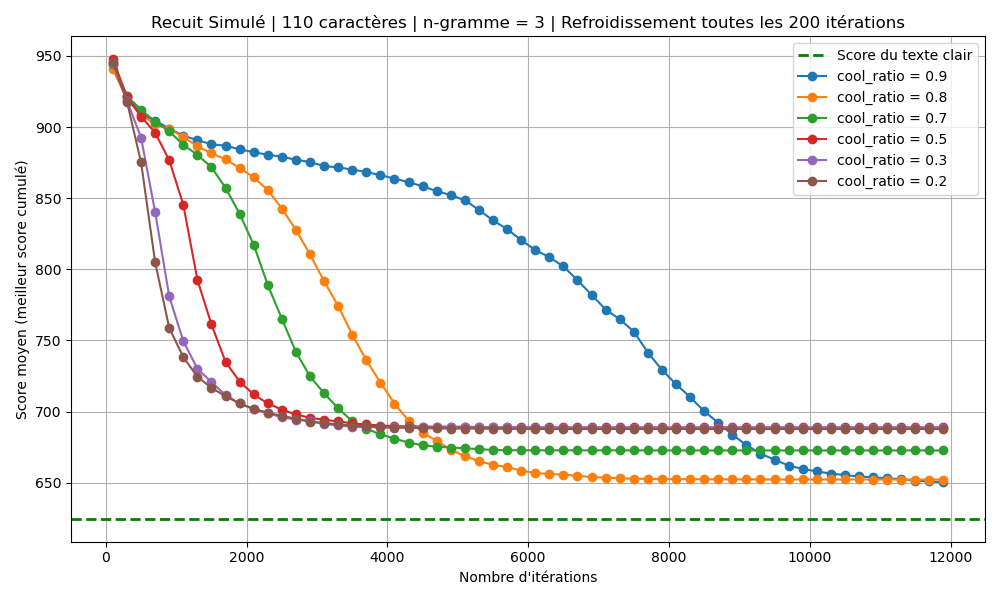
\includegraphics[width=\textwidth]{graphe_recuit_n_3_110_cool_time_200.png}
        \caption{\(\text{Cool\_time}\) = 200 itérations}
        \label{fig:n3-110-200}
    \end{subfigure}
    \hfill
    \begin{subfigure}[b]{0.49\textwidth}
        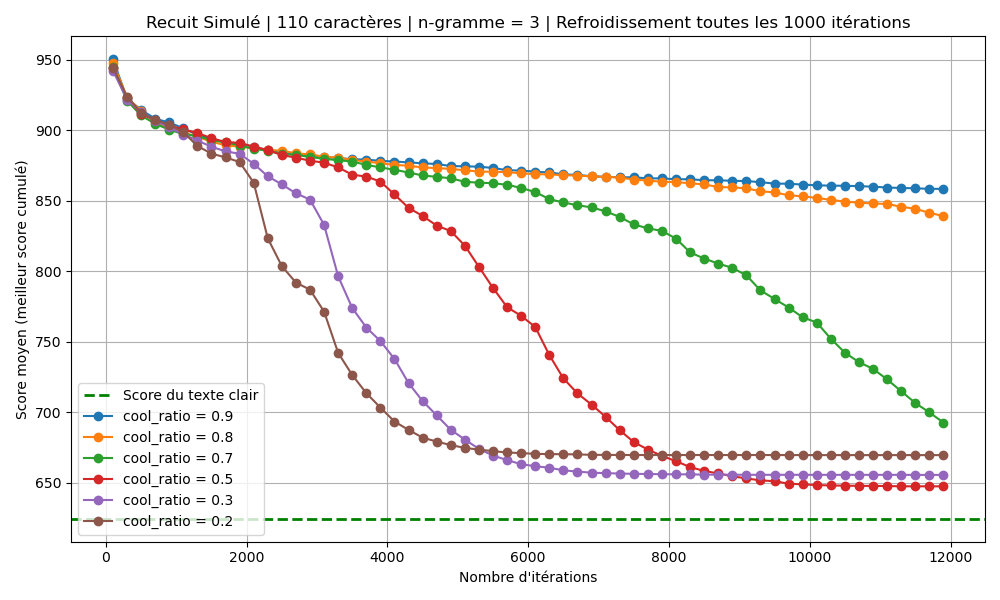
\includegraphics[width=\textwidth]{graphe_recuit_n_3_110_cool_time_1000.png}
        \caption{\(\text{Cool\_time}\) = 1000 itérations}
        \label{fig:n3-509-200}
    \end{subfigure}
    \caption{Texte court (110 caractères)}
    \label{fig:rs-n3-110}
\end{figure}

\begin{itemize}
    \item Pour un refroidissement fréquent (\(\text{cool\_time}\) = 200), on observe qu'un \textit{\(\text{cool\_ratio}\)} bas (par exemple, 0.2 ou 0.3) refroidit rapidement le système. Cela conduit à une convergence précoce vers des scores inférieurs à celui du texte clair, probablement en piégeant l'algorithme dans des minima locaux. 
          En revanche, avec un \(\text{cool\_ratio}\) plus élevé (0.8 ou 0.9), la température décroît lentement, permettant à l’algorithme de continuer à accepter des solutions moins bonnes pendant un plus grand nombre d’itérations, avant de se stabiliser sur une solution assez proche du texte clair. 
          On voit clairement que la valeur \textbf{\(\text{cool\_ratio}\) = 0.8} donne de meilleurs résultats, à partir de 7000 itérations.
    \item Pour un refroidissement moins fréquent (\(\text{cool\_time}\) = 1000), on observe que la décroissance est plus lente, moins immédiate mais finit pas converger. Un \(\text{cool\_ratio}\) élevé (0.8 ou 0.9) retarde la diminution de la température sur le long terme, ce qui donne une impression de stagnation du score moyen, sans aucune amélioration significative.
          Par contre un \(\text{cool\_ratio}\) plus bas (0.2 ou 0.3), permet une décroissance rapide mais contrôlée (à cause de la fréquence réduite) de la température et donc du score moyen. Cela permet à l'algorithme de continuer à explorer l'espace de recherche pendant un plus grand nombre d'itérations et de mener à des scores finaux meilleurs. 
          On remarque qu'un \(\text{cool\_ratio}\) de 0.3 apparaît comme un bon compromis en convergeant vers un score proche du score du texte clair dès environ 7000 itérations, tout en restant comparable aux performances obtenues avec un \(\text{cool\_ratio}\) de 0.5 à 10000 itérations.
\end{itemize}

Dans la suite des comparaisons, nous allons considérer un refroidissement fréquent (\(\text{cool\_time}\) = 200) car il donne de meilleurs résultats en terme de stabilité.

\begin{figure}[H]
    \centering
    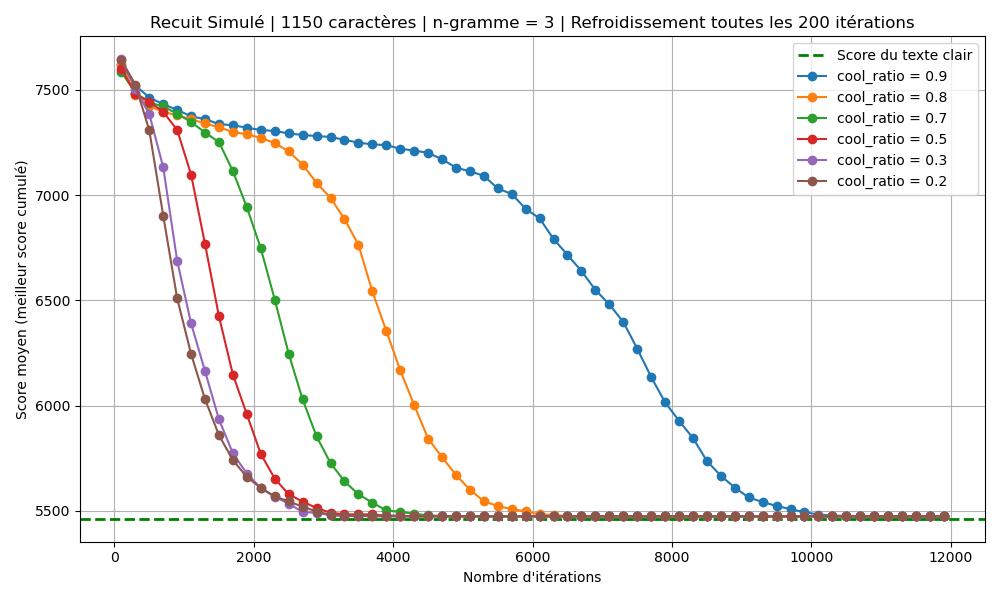
\includegraphics[width=0.8\textwidth, keepaspectratio, height=0.6\textheight]{graphe_recuit_n_3_1150_cool_time_200.png}
    \caption{Texte long (1150 caractères)}
    \label{fig:n3-110-1000}
\end{figure}

On remarque que les graphes ont la même allure, que ce soit pour un texte court ou long. La différence est que la courbe des scores moyens (peu importe la valeur de \(\text{cool\_ratio}\)) se rapproche beaucoup plus du score du texte clair pour le texte long.
On en déduit que le recuit simulé est plus efficace sur des textes longs, tout comme avec les deux algorithmes précédents.


En ce qui concerne l'influence du choix des n-grammes, on note une légère amélioration de la convergence du score moyen les bigrammes ($n=2$). Mais les tétragrammes ($n=4$) ne semblent pas apporter d'amélioration significative (voire même dégradent les performances pour les textes courts). 
Les figures \ref{fig:rs-n2-n4-110} et \ref{fig:rs-n2-n4-1150} en \hyperref[sec:annexes]{annexes} le montrent clairement. Les trigrammes restent une fois de plus le bon compromis pour tous les textes.

Généralement, à  partir de 200-300 caractères, on obtient d'excellents avec le recuit simulé.

\begin{figure}[H]
    \centering
    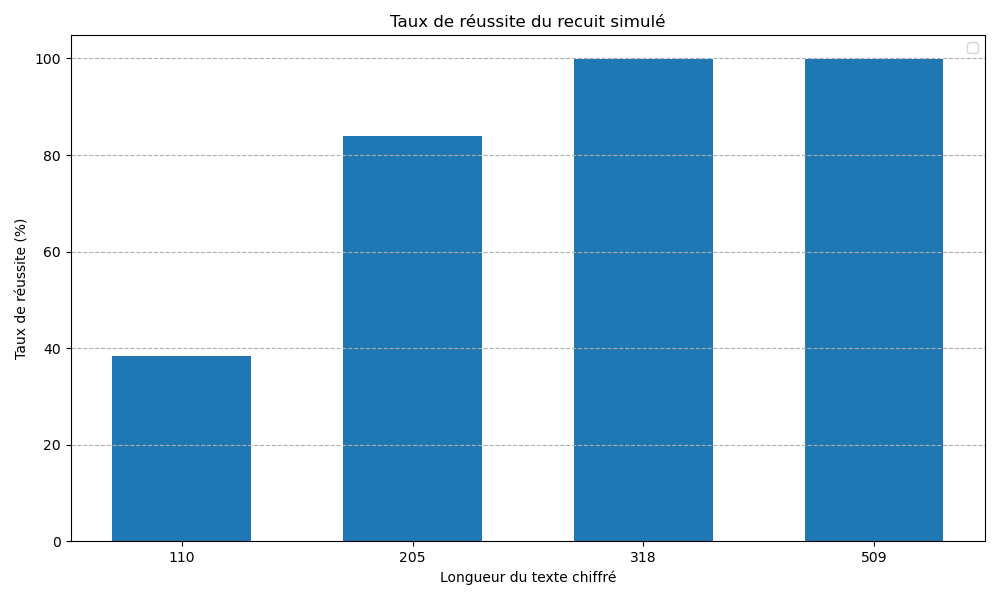
\includegraphics[width=0.7\textwidth, keepaspectratio, height=0.6 \textheight]{taux_reussite_rs.png}
    \caption{Taux de réussite du recuit simulé selon la longueur du texte.}
    \label{fig:taux_reussite_rs}
\end{figure}


\subsection{Recherche tabou}
\subsubsection{Principe de l’algorithme}
La recherche tabou utilise une mémoire pour éviter de revisiter des solutions déjà explorées. L'idée générale est la suivante:

\begin{enumerate}
    \item \textbf{Initialisation:}
    \begin{enumerate}
        \item Partir d'une clé aléatoire $C1$ et l'utiliser pour déchiffrer le cryptogramme.
        \item Calculer le score du texte obtenu.
        \item Initialiser une liste tabou vide, qui servira à mémoriser les solutions explorées.
    \end{enumerate}
    \item \textbf{Boucle principale:}
    \begin{enumerate}[label= (\alph*)]
        \item Explorer un échantillon de clés voisines $C2$ en faisant de légères modifications (voir~\ref{modification_cle}).
        \item Vérifier si $C2$ est dans la liste tabou. Si oui, rejeter la solution
        \item Sinon, calculer le score de $C2$. Si ce score est meilleur que le score précédent, adopter cette nouvelle clé comme clé courante : $C1 \leftarrow C2$.
        \item Ajouter $C2$ à la liste tabou 
    \end{enumerate}
    \item \textbf{Critère d'arrêt:} Terminer l'algorithme après un nombre prédéfini d'itérations.
\end{enumerate}

Les voisins de la clé courante sont générés en permutant deux lettres aléatoires. À chaque itération, un sous-ensemble de 100 clés voisines est sélectionné de manière aléatoire. Cette méthode permet un bon compromis entre diversité des propositions et temps de calcul raisonnable.

\vspace{0.5em}

La liste tabou est implémentée comme un ensemble contenant les clés déjà explorées, représentées sous forme de chaînes de caractères. Dans nos expérimentations, nous avons choisi d’utiliser une liste tabou de taille illimitée. Cela signifie qu’aucune solution ne peut être revisitée une fois marquée comme taboue, même après de nombreuses itérations.
Cette stratégie maximise l’exploration de l’espace des clés, au prix d’un temps d’exécution plus long. Elle agit comme une forme implicite de diversification, forçant l’algorithme à s’éloigner progressivement de la solution initiale. En contrepartie, il devient impossible de revenir sur une bonne solution précédemment écartée. Toutefois, sur des clés de taille modeste (26 lettres), cette stratégie s’est révélée efficace et n’a pas conduit à des impasses, même sur de longues séquences d’itérations.

\vspace{0.5em}

Enfin, on note que la recherche tabou a peu de paramètres à ajuster, ce qui en fait une méthode robuste et relativement simple à implémenter. En dehors du nombre d’itérations et de la stratégie de voisinage, elle ne nécessite pas de réglages fins comme c’est le cas pour d’autres métaheuristiques (par exemple le recuit simulé).


\subsubsection{Résultats}

Nous avons testé l’algorithme pour differentes tailles de texte en utilisant des trigrammes ($n = 3$). La figure~\ref{fig:tabou_taille} montre l’évolution du score moyen au fil des itérations pour 200 essais indépendants.

\begin{figure}[H]
    \centering
    \begin{subfigure}[b]{0.45\textwidth}
        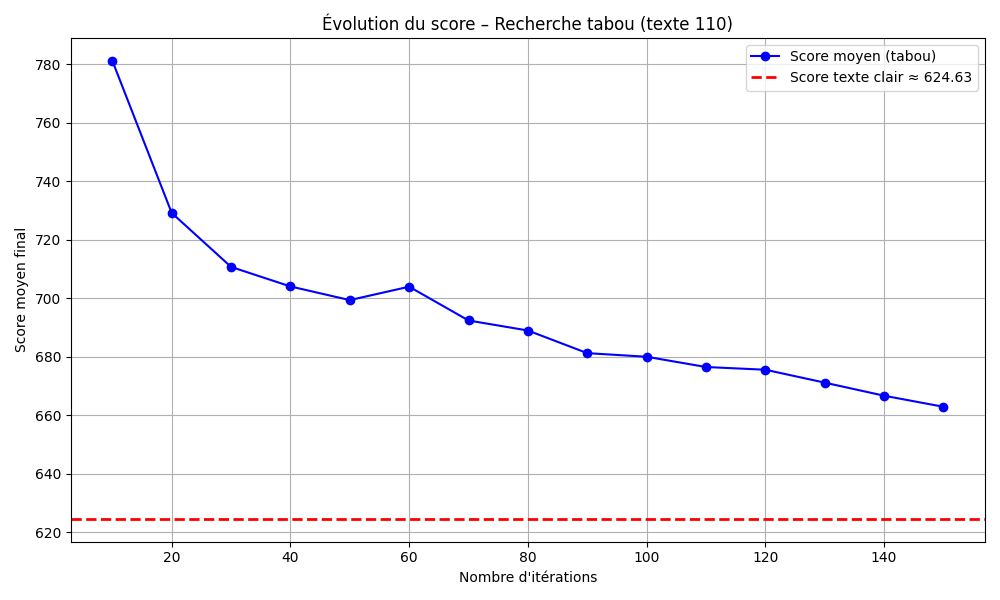
\includegraphics[width=\textwidth]{courbe_tabou_110.png}
        \caption{Texte court : 110 caractères}
    \end{subfigure}
    \hfill
    \begin{subfigure}[b]{0.45\textwidth}
        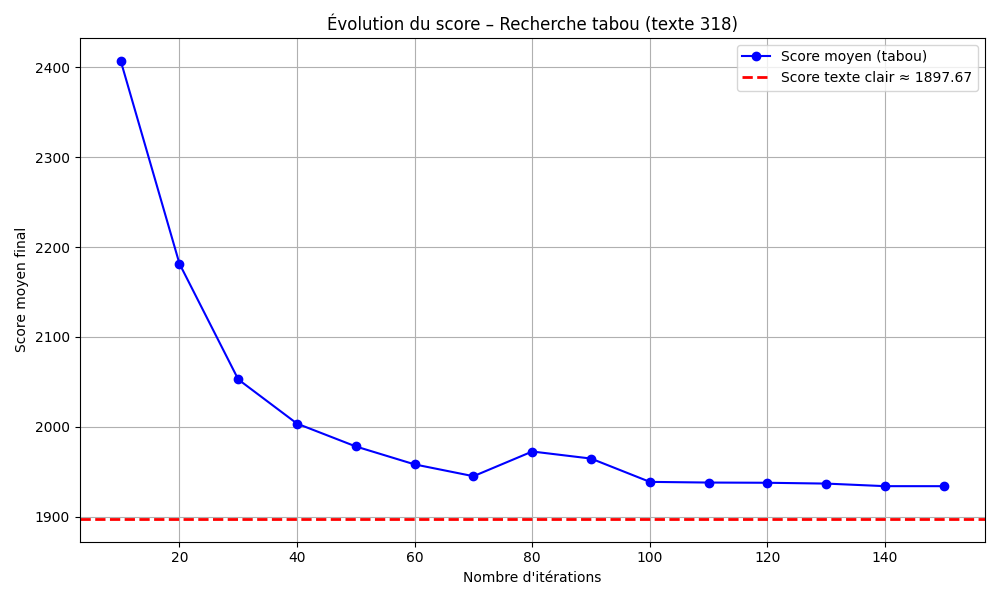
\includegraphics[width=\textwidth]{courbe_tabou_318.png}
        \caption{Texte moyen : 318 caractères}
    \end{subfigure}
    \caption{Évolution du score moyen avec $n = 3$ selon la taille du texte (recherche tabou).}
    \label{fig:tabou_taille}
\end{figure}

On constate, comme pour le \textit{hill climbing}, que les performances augmentent nettement avec la taille du texte. À 110 caractères, les résultats sont très variables d’un essai à l’autre, tandis qu’à partir de 200 caractères, les scores deviennent plus réguliers et plus proches du texte clair. Au-delà de 300 caractères, ce phénomène se stabilise, et les gains sont faibles, ce qui nous conduit à considérer 300 caractères comme une taille suffisante pour obtenir des résultats fiables avec cette méthode. C'est en effet ce nous confirme la figure~\ref{annexe:tabou_500} en \hyperref[sec:annexes]{annexes}.

\medskip

La figure~\ref{fig:tabou_taux} présente le taux de réussite (plus de détails en \ref{sec:Taux_de_réussite}) de la recherche tabou en fonction de la taille du texte.

\begin{figure}[H]
    \centering
    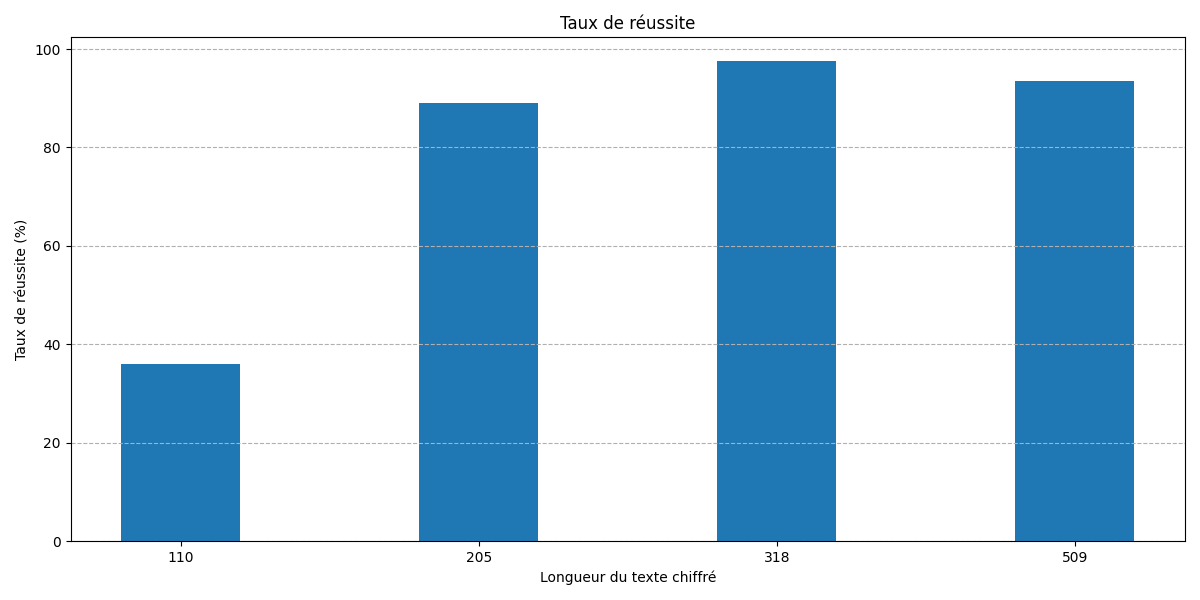
\includegraphics[width=0.8\textwidth]{taux_reussite_tabou.png}
    \caption{Taux de réussite de la recherche tabou selon la taille du texte (avec $n = 3$).}
    \label{fig:tabou_taux}
\end{figure}

On observe une nette progression du taux de réussite avec la taille du texte. Les performances restent modestes pour les très courts messages, mais reste quand même bien plus efficaces que le \textit{hill climbing}.

\section{Comparaisons des différentes métaheuristiques}
\label{sec:comparaison_meta}
Dans cette section, nous allons comparer les performances des quatre algorithmes implémentés en nous basant sur trois indicateurs: la vitesse de convergence du score, le temps d’exécution et le taux de réussite.

\subsection{Vitesse de convergence et temps d'exécution}

Pour faciliter une comparaison visuelle, nous avons appliqué un padding aux courbes de \textit{hill climbing} classique, \textit{hill climbing} optimisé et recuit simulé (8000 permutations) afin de les étendre jusqu'aux 15000 permutations 
(150 itérations * 100 permutations) correspondant à la Recherche Tabou. La figure présente l'évolution du score et le temps d'exécution moyen pour les quatre algorithmes sur un texte de 318 caractères, en utilisant des trigrammes ($n=3$).

\begin{figure}[H]
    \centering
    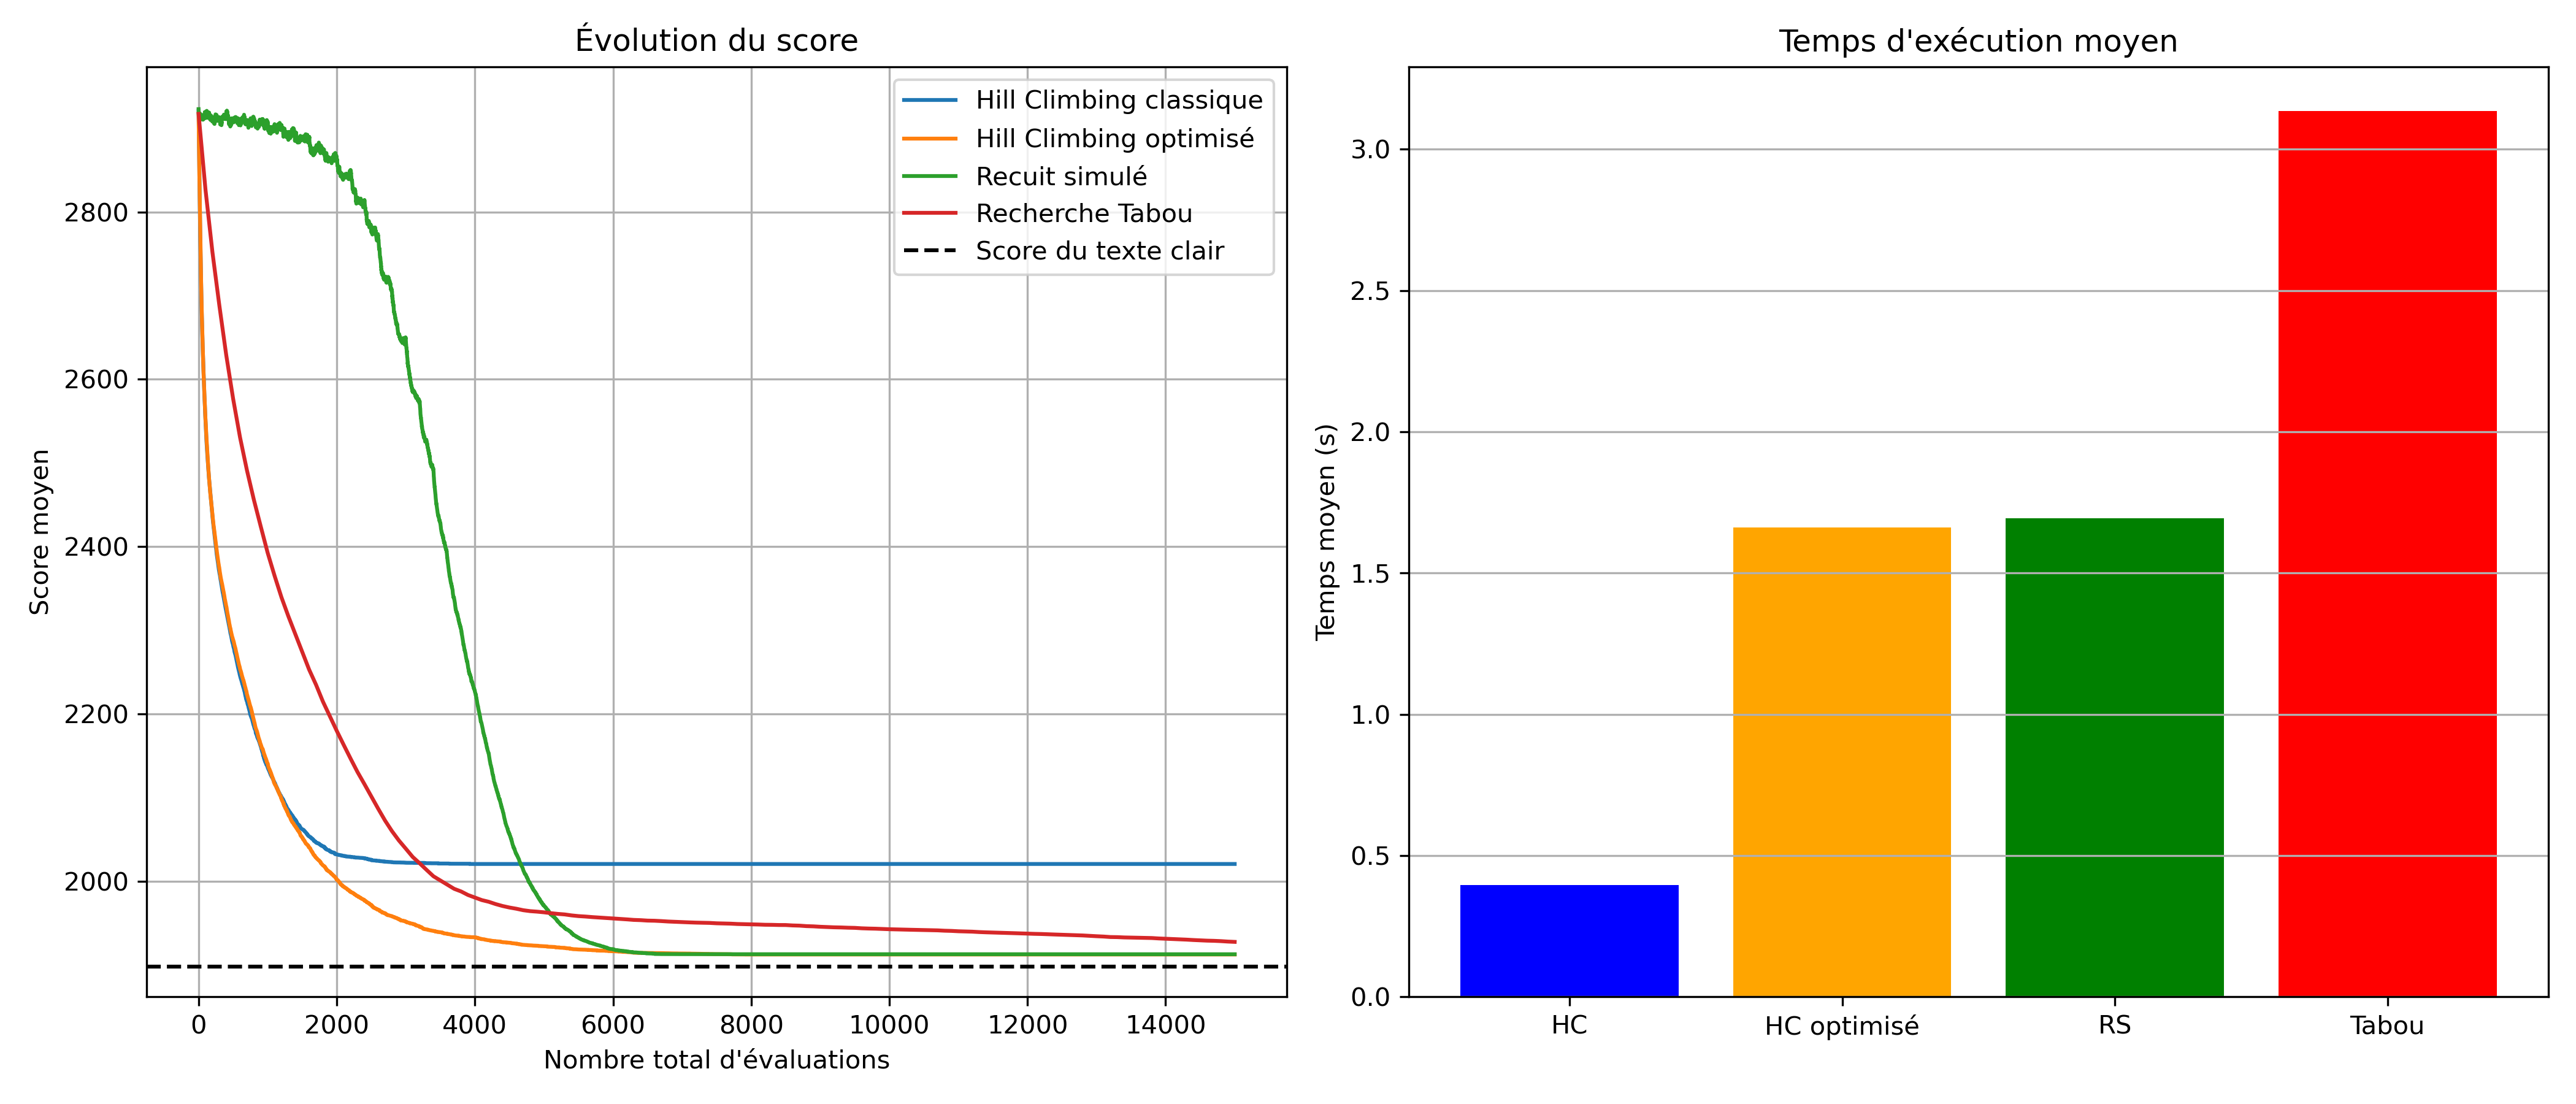
\includegraphics[width=\textwidth, keepaspectratio, height=\textheight]{comparaison_algorithmes_et_temps.png}
    \caption{Comparaison de l'évolution du score et du temps d'exécution moyen}
    \label{fig:score-temps}
\end{figure}

Il apparaît que les variantes du hill climbing (classique et optimisé) amorcent une descente rapide du score dès les premiers instants. Cependant, le hill climbing classique converge de façon \textbf{précoce} et se stabilise rapidement, indiquant une tendance à se bloquer dans des minima locaux. 
A l'inverse, la version optimisée a une convergence plus \textbf{contrôlée} et atteint quasiment le score du texte clair.

Le recuit simulé et la recherche tabou présentent une convergence moins agressive au début, accompagnée d'une exploration plus douce (particulièrement pour le recuit simulé) et d'une amélioration graduelle. Les courbes associées finissent par atteindre un plateau très proche du score du texte clair.


Concernant le temps d'exécution, aucune surprise: le hill climbing classique s'avère le plus rapide, suivi de sa version optimisée et du recuit simulé (ces deux derniers affichant des temps similaires). la Recherche Tabou prend significativement plus de temps en raison de son champ de recherche plus large
et de sa mémoire qu'elle doit parcourir à chaque itération.

\subsection{Taux de réussite}
\label{sec:Taux_de_réussite}

Nous allons d'abord définir l'indice de lisibilité noté \textbf{idl} du message déchiffré. Cet indice, qui varie entre 0 (texte illisible) et 1 (texte parfaitement lisible), est calculé à partir de la correspondance entre le dictionnaire de chiffrement réel et celui obtenu par cryptanalyse, en pondérant chaque lettre par sa fréquence en français. 
La formule utilisée est la suivante :

\[
idl = \sum_{c \in \mathcal{A}} p(c) \cdot \delta\Bigl(\texttt{dico\_trouve}(c) = \texttt{dico\_reel}(c)\Bigr)
\]


où :
\begin{itemize}
  \item \(\mathcal{A}\) est l'ensemble des lettres de l'alphabet,
  \item \(p(c)\) est la fréquence d'apparition de la lettre \(c\) en français,
  \item \(\delta(\cdot)\) est la fonction indicatrice qui vaut 1 si la condition est vérifiée et 0 sinon.
\end{itemize}

Pour les besoins de ce projet, cette formule repose sur l'hypothèse que nous disposons de la clé de chiffrement, ce qui n'est pas toujours le cas en pratique.
On ne se contente pas de compter le nombre de lettres correctement identifiées; chaque correspondance est pondérée par l'importance statistique de la lettre. Ainsi, ne pas trouver le bon correspondant pour une lettre peu fréquente (par exemple, la lettre "w") aura un impact limité sur l'indice idl, alors que l'absence d'une lettre très fréquente (comme "E") pénalisera fortement le score.

Pour qualifier une cryptanalyse de \og réussie \fg{}, on considère que l'indice de lisibilité idl doit être supérieur à 0.9 (90\%). Le taux de réussite d'un algorithme donné est calculé en comptant le nombre de cryptanalyse ayant \og réussie \fg{} sur 500 exécutions indépendantes et pour chaque taille de texte. Les résultats sont présentés sur la figure \ref{fig:tous-reussite}.

\begin{figure}[H]
    \centering
    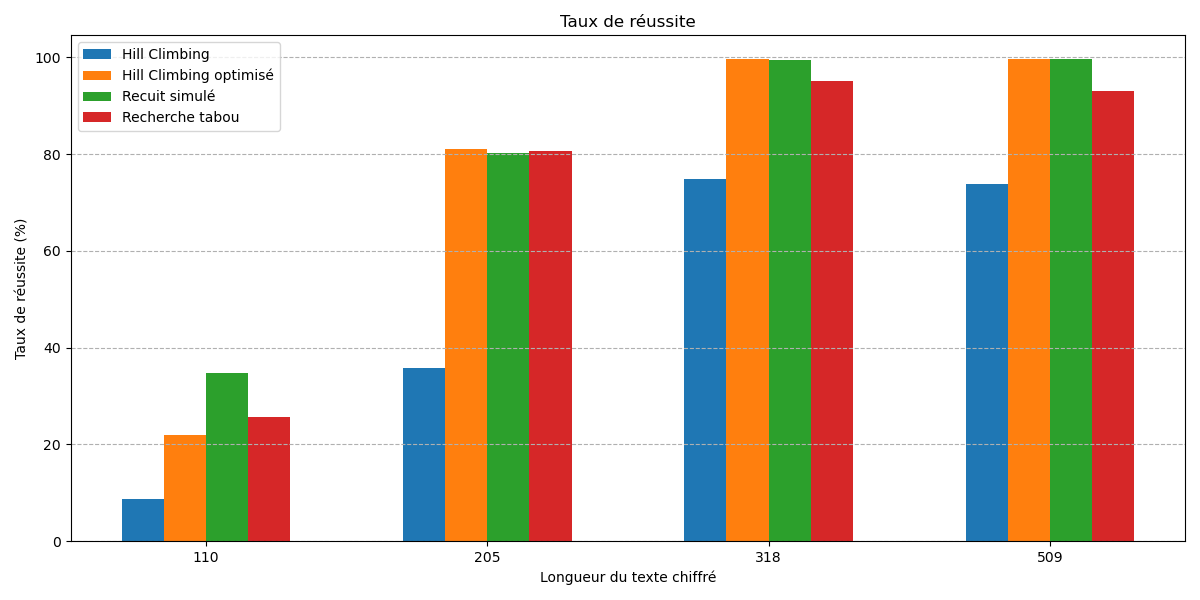
\includegraphics[width=\textwidth, keepaspectratio, height=\textheight]{taux_reussite.png}
    \caption{Taux de réussite des algorithmes selon la longueur du texte.}
    \label{fig:tous-reussite}
\end{figure}

On observe que pour les textes courts (jusqu'à 110 caractères), les quatre méthodes sont peu efficaces. À partir de 200 caractères, une nette amélioration du taux de réussite est constatée, atteignant environ 80\% pour la plupart des algorithmes, à l'exception du hill climbing classique qui plafonne autour de 40\%. Pour des textes de 300 caractères et plus, d'excellents résultats sont obtenus, 
avec un taux de réussite supérieur à 90\% pour le recuit simulé, le hill climbing optimisé et la Recherche Tabou.\\
Verdict final: En termes d'efficacité et de rapidité d'exécution, le \textit{hill climbing} optimisé et le recuit simulé représentent les meilleurs compromis, particulièrement lorsque la longueur du texte est assez importante.


\section{Limites de l'attaque par analyse fréquentielle}

Bien qu'efficace sur le chiffrement par substitution, l'attaque par analyse fréquentielle montre rapidement ses limites face à certains cas particuliers. En voici quelques exemples notables:
\begin{itemize}
    \item \textbf{Longueur insuffisante du texte}: Comme on a pu le souligner plus haut, les textes courts ne fournissent pas assez de données statistiques pour que l'analyse fréquentielle soit fiable.
    \item \textbf{Structures linguistiques atypiques}: Certains textes littéraires exploitent des contraintes formelles qui brouillent les statistiques usuelles. 

    \underline{Premier exemple}:\\

    \textit{La Disparition} de Georges Perec est un roman \textbf{lipogramme} de 300 pages dans lequel n'apparaît que cinq fois la lettre \og e \fg{}, pourtant la plus fréquente en français. En voici un extrait:

    \begin{quote}
        \textit{Anton Voyl n’arrivait pas à dormir. Il alluma. Son Jaz marquait minuit vingt. Il poussa un profond soupir, s’assit dans son lit, s’appuyant sur son polochon. Il prit un roman, il l’ouvrit, il lut ; mais il n’y saisissait qu’un imbroglio confus, il butait à tout instant sur un mot dont il ignorait la signification...}
    \end{quote}

    L’analyse des fréquences fait disparaître le \og e \fg{} et rend donc l'identification à un texte de la langue française difficile.\\

    \underline{Deuxième exemple}:

    \begin{quote}
        \textit{De Zanzibar à la Zambie et au Zaïre, des zones d’ozone font courir les zèbres en zigzags zinzins.}
    \end{quote}

    Ici, c’est la surabondance de la lettre \og Z \fg{} qui pose problème.

\end{itemize}

\section{Conclusion}

Ce projet a permis d’explorer différentes approches de cryptanalyse automatisée du chiffrement par substitution monoalphabétique. Nous avons implémenté plusieurs métaheuristiques — \textit{hill climbing}, recuit simulé, recherche tabou — et les avons évaluées de manière comparative selon des critères de performance, tels que le taux de réussite, la stabilité et le temps d’exécution.

Si le \textit{hill climbing} classique constitue une solution simple et rapide, il souffre de blocages fréquents dans des minima locaux. Pour pallier cette faiblesse, une version optimisée introduisant des redémarrages aléatoires s’est révélée bien plus robuste, notamment sur les textes courts. Le recuit simulé et la recherche tabou, quant à eux, se sont montrés particulièrement efficaces dès que la taille du texte permet une exploitation fiable des statistiques n-grammiques. Parmi les configurations testées, l’utilisation de trigrammes a offert un bon compromis entre précision et régularité.

Néanmoins, l’analyse fréquentielle montre rapidement ses limites dans certains contextes : textes trop courts, constructions linguistiques atypiques, ou distributions de lettres volontairement perturbées. C’est pourquoi d’autres types d’attaques peuvent s’avérer plus pertinents selon les situations. L’\textit{attaque par mot probable}, par exemple, repose sur l’hypothèse de la présence d’un mot attendu dans le message. Elle a joué un rôle historique décisif contre la machine \textit{Enigma}, lorsque les cryptanalystes britanniques ont exploité l’occurrence fréquente du mot \og Führer \fg{} dans les messages allemands. En conjuguant cette stratégie à une analyse structurelle et à des erreurs humaines, ils ont réussi à briser le chiffrement d’Enigma — un événement qui a profondément influencé le cours de la Seconde Guerre mondiale.

Ce projet ouvre ainsi la voie à de nombreuses perspectives. D’abord, il serait possible d’explorer d’autres types d’algorithmes, ou même d’en combiner plusieurs pour tirer parti de leurs forces respectives. On pourrait aussi appliquer ces méthodes à des systèmes de chiffrement plus complexes, comme le chiffre de Vigenère, les grilles de transposition, ou encore des machines historiques comme Enigma.

Enfin, dépasser la simple analyse des fréquences permettrait de rendre les attaques plus efficaces dans des situations réalistes : par exemple en s’appuyant sur des outils de traitement automatique de la langue, capables de reconnaître des structures grammaticales, ou en prenant en compte les erreurs ou les abréviations présentes dans les messages. Cela permettrait de mieux s’adapter à la variété des textes rencontrés dans des contextes réels.


\clearpage
\section*{Annexes}

\begin{figure}[H]
    \centering
    \begin{subfigure}[b]{0.49\textwidth}
        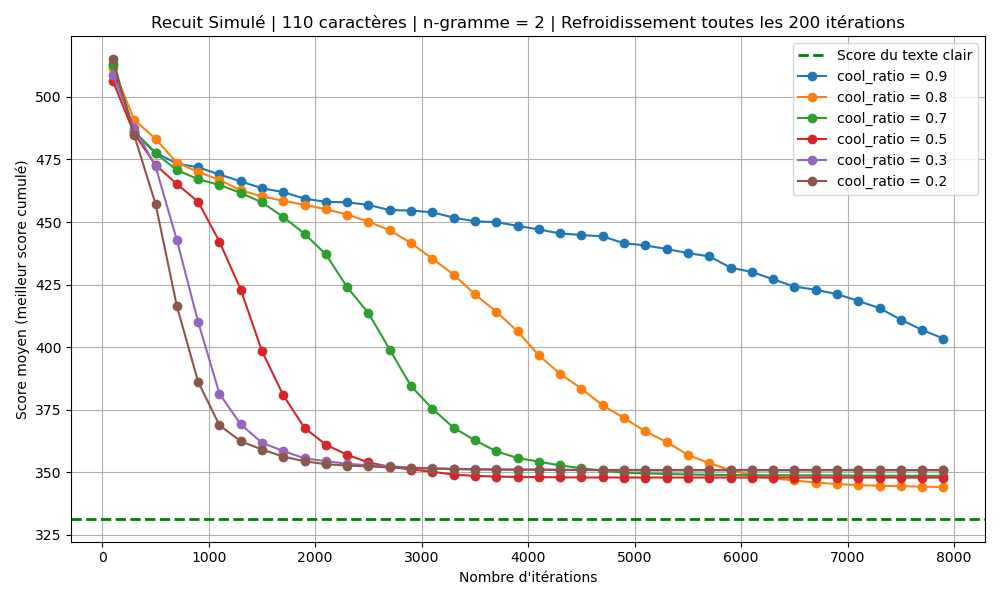
\includegraphics[width=\textwidth]{graphe_recuit_n_2_110_cool_time_200.png}
        \caption{n = 2}
        \label{fig:n2-110-200}
    \end{subfigure}
    \hfill
    \begin{subfigure}[b]{0.49\textwidth}
        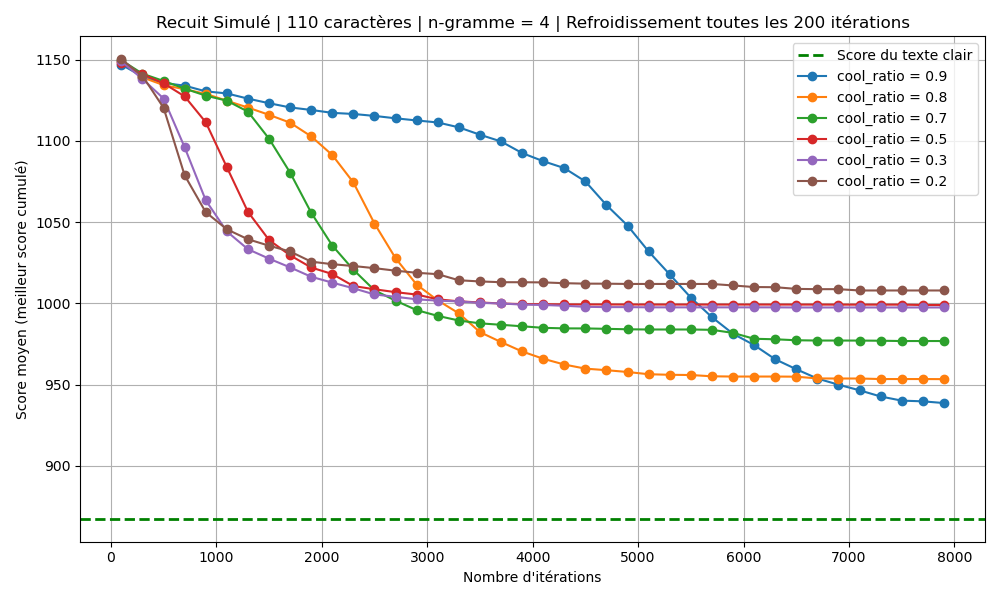
\includegraphics[width=\textwidth]{graphe_recuit_n_4_110_cool_time_200.png}
        \caption{n = 4}
        \label{fig:n4-110-200}
    \end{subfigure}
    \caption{Influence des n-grammes. Texte court (110 caractères) avec recuit simulé.}
    \label{fig:rs-n2-n4-110}
\end{figure}

\begin{figure}[H]
    \centering
    \begin{subfigure}[b]{0.49\textwidth}
        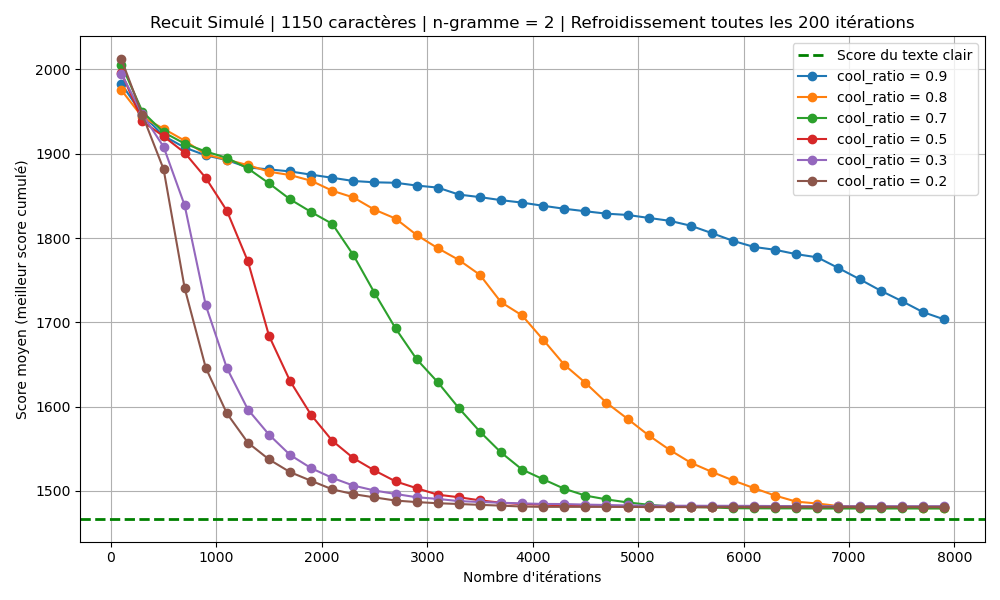
\includegraphics[width=\textwidth]{graphe_recuit_n_2_1150_cool_time_200.png}
        \caption{n = 2}
        \label{fig:n2-1150-200}
    \end{subfigure}
    \hfill
    \begin{subfigure}[b]{0.49\textwidth}
        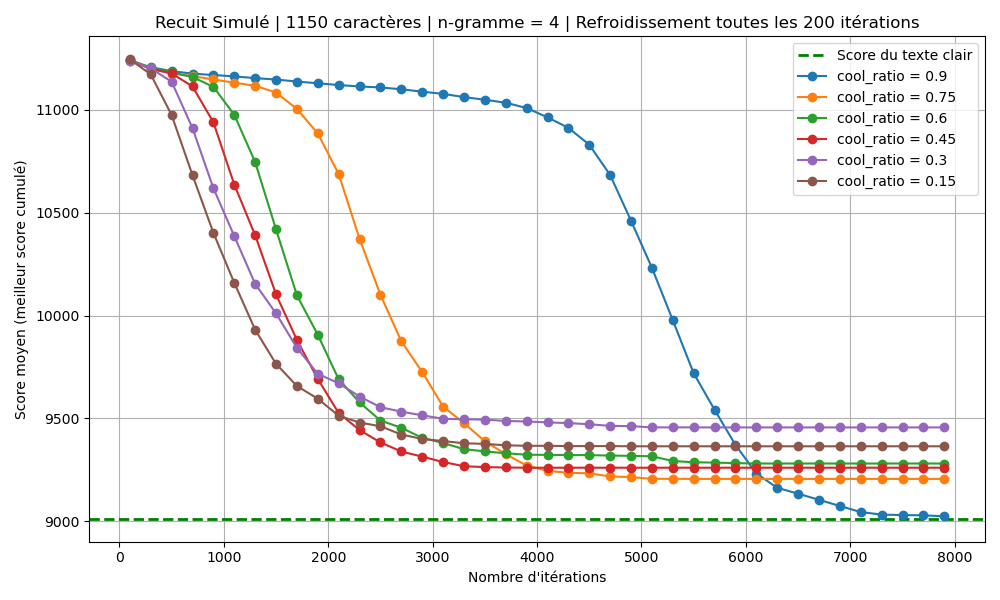
\includegraphics[width=\textwidth]{graphe_recuit_n_4_1150_cool_time_200.png}
        \caption{n = 4}
        \label{fig:n4-1150-200}
    \end{subfigure}
    \caption{Influence des n-grammes. Texte long (1150 caractères) avec recuit simulé.}
    \label{fig:rs-n2-n4-1150}
\end{figure}
\begin{figure}[H]
    \centering
    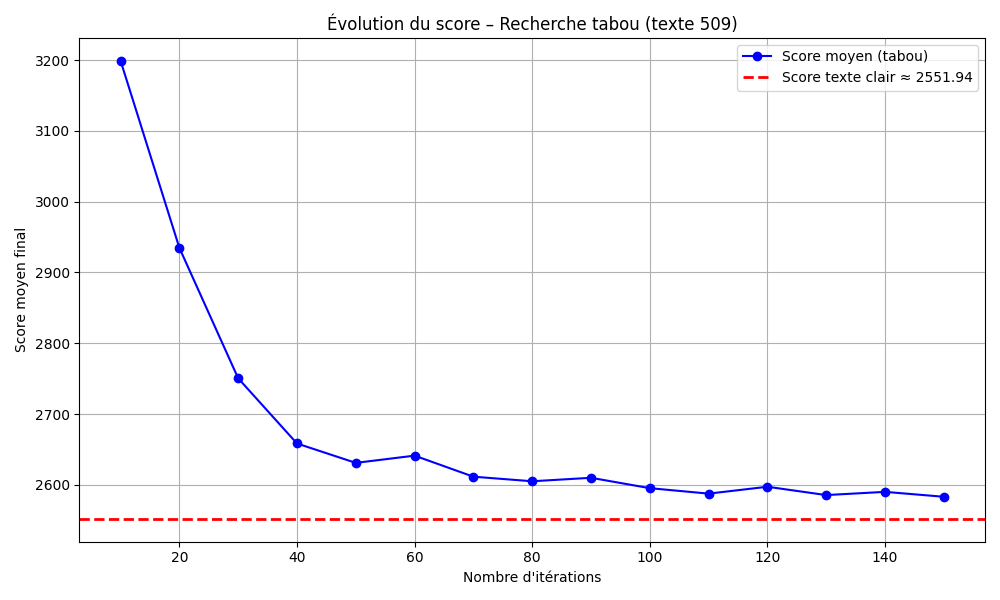
\includegraphics[width=0.7\textwidth]{courbe_tabou_509.png}
    \caption{Évolution du score moyen pour un texte de 509 caractères avec $n = 3$ (recherche tabou).}
    \label{annexe:tabou_500}
\end{figure}


\clearpage
\addcontentsline{toc}{section}{Annexes}\label{sec:annexes}
\section*{Références}

\begin{enumerate}[label={[\arabic*]}]
    \item Page web Bibmath, \url{https://www.bibmath.net/crypto/}
    \item Didier Müller, \textit{Les métaheuristiques en cryptanalyse},  Bulletin no 143 de la \href{https://www.vsmp.ch/}{SSPMP}, mai 2020, \url{https://www.apprendre-en-ligne.net/auteur/articles/metaheuristiques-cryptanalyse.pdf}
    \item \textit{Automated cryptanalysis of substitution cipher using hill climbing}, \url{https://www.montis.pmf.ac.me/vol44/11.pdf}
    \item Helder Brito, O'nel Hounnouvi, \textit{Dépôt GitHub du projet}, \url{https://github.com/onelhounnouvi/LU2IN013-Projet}
\end{enumerate}

\end{document}